\documentclass{article}

% Boilerplate {{{

\usepackage{amsmath}
\usepackage{unicode-math}
\setmainfont{XITS}
\setmathfont{XITS Math}
\usepackage{tikz}
\usetikzlibrary{matrix}
\usepackage{newunicodechar}
\usepackage{galois}
\usepackage{amsthm}

\theoremstyle{definition}
\newtheorem*{definition}{Definition}
\newtheorem*{example}{Example}

\theoremstyle{plain}
\newtheorem*{lemma}{Lemma}
\newtheorem{theorem}{Theorem}
\newtheorem{corrolary}{Corrolary}

\newcommand{\iif}{\underline{\text{if}}}
\newcommand{\case}{\underline{\text{case}}}
\newcommand{\halt}{\underline{\text{halt}}}
\newcommand{\lam}{\underline{\text{λ}}}
\newcommand{\add}{\text{add1}}
\newcommand{\sub}{\text{sub1}}
\newcommand{\gez}{\text{gez}}
\newcommand{\INT}{\text{INT}}
\newcommand{\TRUE}{\text{TRUE}}
\newcommand{\FALSE}{\text{FALSE}}
\newcommand{\ddo}{\operatorname{do}}
\newcommand{\llet}{\operatorname{let}}
\newcommand{\return}{\operatorname{return}}
\newcommand{\getstore}{\operatorname{get-σ}}
\newcommand{\putstore}{\operatorname{put-σ}}
\newcommand{\getenv}{\operatorname{get-ρ}}
\newcommand{\putenv}{\operatorname{put-ρ}}
\newcommand{\gettime}{\operatorname{get-τ}}
\newcommand{\puttime}{\operatorname{put-τ}}
\newcommand{\coercebool}{\operatorname{↓𝔹}}
\newcommand{\coercekon}{\operatorname{↓λ₁}}
\newcommand{\coercefun}{\operatorname{↓λ₂}}
\newcommand{\liftpowerset}{\operatorname{↑𝒫}}
\newcommand{\touchedcall}{\operatorname{𝓉𝒞}}
\newcommand{\touchedvar}{\operatorname{𝓉Var}}

\newcommand{\C}{L}
\newcommand{\A}{\widehat{L}}

\newcommand{\Csteps}{↦}
\newcommand{\Asteps}{\ \widehat{↦}\ }

\newcommand{\Ce}{e}
\newcommand{\Ae}{\widehat{e}}

\newcommand{\AStore}{\widehat{Store}}
\newcommand{\AEnv}{\widehat{Env}}
\newcommand{\ATime}{\widehat{Time}}
\newcommand{\AVal}{\widehat{Val}}

\newcommand{\PM}{𝒫\ }
\newcommand{\PT}{𝒫_T\ }

\newcommand{\SM}{State}
\newcommand{\ST}{State_T}

\newenvironment{donotbreak}
{\\[0.5\baselineskip]\begin{minipage}{\linewidth}}
{\end{minipage}\\[0.5\baselineskip]}

% \usepackage{multicol}

% \newunicodechar{λ}{\lambda}
% \newunicodechar{→}{\rightarrow}
% \newunicodechar{𝒯}{\mathcal{T}}
% \newunicodechar{∀}{\forall}
% \newunicodechar{∘}{\circ}
% \newunicodechar{𝒫}{𝒫\ }


% \usepackage{amssymb}
% \usepackage{listings}
% \usepackage{stmaryrd}
% \usepackage{wasysym}
% \usepackage{cite}
% \usepackage{pgfplots}
% \usepackage{minted}
% \usepackage{float}
% \usepackage{caption}
% \usepackage{fontspec}
% \setmonofont{Inconsolata}
% % \usepackage{hyperref}
% 
% \lstset{basicstyle=\footnotesize\ttfamily,language=haskell}
% \lstMakeShortInline|
% 
% \newmintedfile[haskell]{haskell}{}
% \newmintinline[h]{haskell}{}
% \newmintinline[p]{text}{}
% 
% \newenvironment{itemizenobreak}
% {\\[0.5\baselineskip]\begin{minipage}{\linewidth}\begin{itemize}}
% {\end{itemize}\end{minipage}\\[0.5\baselineskip]}
% 
% 
% \newcommand{\DSS}{\text{\lstinline|SS|}}
% \newcommand{\DSSAbs}{\widehat{\text{\lstinline|SS|}}}
% \newcommand{\Dstep}{\text{\lstinline|step|}}
% \newcommand{\DstepAbs}{\widehat{\text{\lstinline|step|}}}
% 
% %%% pulled from internet (stack overflow user Christian Feuersänger) %%%
% % argument #1: any options
% \newenvironment{customlegend}[1][]{%
%     \begingroup
%     % inits/clears the lists (which might be populated from previous
%     % axes):
%     \csname pgfplots@init@cleared@structures\endcsname
%     \pgfplotsset{#1}%
% }{%
%     % draws the legend:
%     \csname pgfplots@createlegend\endcsname
%     \endgroup
% }%
% 
% % makes \addlegendimage available (typically only available within an
% % axis environment):
% \def\addlegendimage{\csname pgfplots@addlegendimage\endcsname}
% 


\title{Abstract Control in Static Analysis}
\author{David Darais}
\date{\today}

\begin{document}
\maketitle

% }}}

% Abstract {{{
\begin{abstract}

The field of static analysis offers many techniques for automatically discovering facts about programs.
For example, a static analysis might be used to verify that a program is memory safe, or that it obeys a privacy policy.
Techniques based on Abstract Interpretation (AI) allow the analysis designer to vary some properties of an analysis.
However, features like context, object, and flow sensitivity are often hard-coded into an analysis based on classic AI.
Abstracting Abstract Machines (AAM) is one design methodology for analysis which exposes more of these features as tuning knobs.
Unfortunately, AAM lacks reusable tools for building analyses, and not all analysis features fit nicely into the framework.

We propose a new compositional framework for designing analyses which support a tuning knob missing from AAM: abstract control.
We achieve compositionality by refactoring AAM into monad transformers, each of which we relate back to abstract state machines piecewise.
When put together, these monad transformers build analyses which are correct by construction.
Furthermore, the monadic abstraction allows us to recover a new tuning knob which we call abstract control.
Abstract control allows one to adjust the flow and path sensitivity of an analysis independent of other design choices.

\end{abstract}
% }}}

\tableofcontents

% Introduction {{{
\section{Introduction}
\label{Intro}

Static analysis has many applications.
A software developer might use an analysis to find bugs in a program.
A software merchant might use an analysis to detect malware or other security vulnerabilities in software hosted by their app store.
A manufacturer might use an analysis to establish high assurance in the reliability of control software for a car or airplane.
Each of these situations requires a different type of analysis.
To meet the needs of a given problem, an analysis designer has two options: retrofit an existing analysis or design one from scratch.
Retrofitting an existing analysis can be insufficient because the tension between precision and performance is often too high.
Getting an analysis right might require more modification than an existing analysis was designed to support.
Because of this, complex analyses often need to be designed from scratch, and analysis designer need tools to help them with this process.

Designing a static analysis is hard.
Designing \emph{the right} static analysis is even harder.
One possible process for arriving at the right static analysis is:
\begin{enumerate}
\item Describe the semantics of your language.
\item Design an analysis which you hope has right properties.
\item Exercise the analysis.
\item If the analysis is too slow or imprecise: repeat from 2.
\end{enumerate}
To get a complex analysis right this process must be repeated multiple times.
Iterating quickly between the design and exercise of an analysis is the key to getting the analysis you wanted without too much unnecessary effort.

One methodology which aims to ease the design process for static analysis is the Abstracting Abstract Machines (AAM) 
  framework\cite{van-horn:2010:aam}.
AAM separates two design steps which are traditionally tightly coupled: describing features of interest and abstracting those features.
Furthermore, AAM shows that the abstraction step is systematic, freeing the analysis designer to spend effort in designing features of interest.
However, AAM doesn't provide reusable tools for constructing analyses.
The analysis designer must describe their state machine transition function from scratch.
Additionally, some analysis features like flow and path sensitivity don't fit nicely into the AAM framework.

We propose a new compositional framework for designing analyses which supports a tuning knob missing from AAM: abstract control.
To achieve this we refactor AAM into monad transformers.
Using monad transformers, the analysis designer can easily add and remove features from their semantics independently of other features.
The monadic abstraction additionally exposes a new tuning knob for analyses which we call abstract control.
Abstract control allows one to adjust the flow and path sensitivity of an analysis independent of other design choices.

To justify the soundness of the approach, we show that the monad transformers we use are also Galois connection transformers.
This means that any combination of our monad transformers will yield a sound approximation of a state machine semantics.

Our contributions in this work are:
\begin{enumerate}
\item A monadic formulation of AAM which exposes abstract control as a tuning knob.
\item A compositional analysis \emph{implementation} framework for building abstract state machines using monad transformers.
\item A compositional analysis \emph{proof} framework for justifying the correctness of abstract state machines using Galois connection transformers.
\item A new monad transformer for nondeterminism which serves as our gateway to recovering abstract control as a tuning knob.
\end{enumerate}

The rest of the paper is structured as follows:
Section \ref{Background} covers necessary background material in semantics, analysis, and the CPS language which we use for examples.
Section \ref{CompositionalAnalysis} demonstrates a monadic variant of AAM which supports defining compositional interpreters for analysis.
Section \ref{AbstractControl} discusses abstract control and how we exploit the monadic abstraction to expose a tuning knob for it.
Section \ref{Optimizations} gives two examples of analysis optimizations and how they adapt seamlessly to variations in abstract control.
Section \ref{Correctness} discusses the correctness framework and what key lemmas are involved.
Section \ref{Proofs} shows proof steps in more detail for the arguments made in section \ref{Correctness}.
Sections \ref{RelatedWork} and \ref{FutureWork} discuss relate and future work, and section \ref{Conclusion} concludes.

% }}}

% Background {{{
\section{Background}
\label{Background}

In this section we discuss background material potentially useful for understanding our compositional analysis framework.
This section provides merely a sketch these concepts, and does not motivate them directly in the context of our work.
Some readers may find it useful to skip ahead to section \ref{CompositionalAnalysis} and chase backlinks as they are needed and motivated.
Or some may prefer to proceed directly with this section, consuming the document in a more bottom-up fashion.
For these readers, we have done our best to keep this section brief.
 
% Small Step Semantics {{{
\subsection{Small-Step Semantics}
\label{SS-Semantics}

We use the small-step operational approach to semantics pioneered by independently by 
  Plotkin\cite{plotkin:1981:sos} 
  and Felleisen\cite{felleisen:1992:red-sem}.
In small-step operational semantics, expressions in a language are given meaning by mapping them to state machines.
Formally, a small-step semantics for a language $L$ is given by:
\begin{itemize}
\item A state machine with configuration states $\C$.
\item A transition relation $σ \Csteps σ'$ for $(\Ce, \Ce' : \C)$.
\item An embedding function $η : L → \C$.
\end{itemize}
The meaning of an expression $e$ is then given by a final configuration $σ$ reachable by $η(e)$ through $\Csteps$.

Small-step semantics contrast to previously developed denotational approaches.
A denotational semantics for a language $L$ is given by a denotation function $⟦\_⟧$ mapping terms $e$ to objects in a mathematical space.
This denotation function can quickly demand non-trivial mathematical machinery for even very simple languages.
Small-step methods side-step the need for such machinery at the cost of potentially useful mathematical structure.
Many useful analysis properties can be states as properties of execution states of an abstract machine.
Small-step semantics therefore serve as a nice middle-ground marrying formality and simplicity.

% }}}

% CPS {{{
\subsection{Continuation Passing Style}
\label{CPS}

We use CPS-IF as an example language to demonstrate our framework.
CPS-IF is a variant of continuation passing style λ-calculus extended with conditionals and branching.
We use λ-calculus because it is the simplest language with support for higher-order control flow.
λ-calculus can serve as the core target language for larger languages which appear in practice.
We use CPS because the state machine for the semantics of CPS requires one less component and it simplifies our presentation.
All lambda calculus terms can be translated to CPS terms through CPS-conversion, so there is no loss in language expressivity.
We add conditionals to help exercise analyses which track branching structure in different ways.

We define the CPS-IF language as follows:
\begin{align*}
x,y,k : Var  &⩴ ...variables...                                          \\
b,i,l : Lit  &⩴ ℤ ∪ 𝔹                                                    \\
  f,g : Lam  &⩴ \lam(x) → e \;|\; \lam(x,k) → e                          \\
    a : Atom &⩴ x \;|\; l \;|\; f \;|\; op(a)                            \\
   op : Op   &⩴ \add \;|\; \sub \;|\; \gez                               \\
    e : Exp  &⩴ \iif(a)\{e\}\{e\} \;|\; a(a) \;|\; a(a,a) \;|\; \halt(a) \\
\end{align*}



CPS-IF supports integer and boolean literals, addition and subtraction by 1, and testing if an integer is greater than or equal to zero.
The essence of CPS is in the syntactic restriction on application forms $a(a)$ and $a(a,a)$.  
Because $a$ cannot be a nested expression, evaluating an $Exp$ requires no evaluation stack.

The state machine $\C$ for CPS-IF is defined as:
\begin{align*}
𝓁 : \CAddr  &≔ ℤ                     \\
ρ : \CEnv   &≔ Var → \CAddr          \\
θ : \CStore &≔ \CAddr → \CVal        \\
v : \CVal   &⩴ l \;|\; ⟨f, ρ⟩        \\
\Ce : \C    &≔ Exp × \CEnv × \CStore \\
\end{align*}


Environments map variables to addresses, and the store maps addresses to values.
Values contain closures, which are lambda expressions paired with their closure environment.

The small-step semantics for CPS-IF are defined in two parts.
First we define a \emph{denotation function} $𝒜 $ for $Atom$ expressions.
\begin{align*}
𝒜                      &: \CEnv × \CStore × Atom ⇀ \CVal                              \\
𝒜 (ρ,θ,x)              &≔ θ(ρ(x))                                                     \\
𝒜 (ρ,θ,l)              &≔ \{ l \}                                                     \\
𝒜 (ρ,θ,\add(a))         &≔ 𝒜 (ρ,θ,a) + 1                                               \\
𝒜 (ρ,θ,\sub(a))         &≔ 𝒜 (ρ,θ,a) - 1                                               \\
𝒜 (ρ,θ,\gez(a))         &≔ \{ True \;\text{if}\; 𝒜 (ρ,θ,a) >= 0, False \;\text{otherwise} \} \\
𝒜 (ρ,θ,\lam(x) → e)    &≔ ⟨\lam(x) → e, ρ⟩                                            \\
𝒜 (ρ,θ,\lam(x)(k) → e) &≔ ⟨\lam(x)(k) → e, ρ⟩                                         \\
\end{align*}



Second we define a \emph{step relation} (as a function) $ℰ$ for $Exp$ expressions.
\begin{align*}
ℰ                            &: Exp × \CEnv × \CStore ⇀  Exp × \CEnv × \CStore                     \\
  ℰ(\iif(a)\{e₁\}\{e₂\},ρ,θ) &≔ \{ (e₁,ρ,θ) \;\text{if}\; 𝒜 (ρ,θ,a) = True, (e₂,ρ,θ) \;\text{if}\; 𝒜 (ρ,θ,a) = False \} \\
            ℰ(a₁(a₂,a₃),ρ,θ) &≔ (e, ρ'', θ'')                                                      \\
                             &\text{where}                                                         \\
        ⟨\lam(x)(k) → e, ρ'⟩ &= 𝒜 (a₁, ρ, θ)                                                       \\
                          v₂ &= 𝒜 (a₂, ρ, θ)                                                       \\
                          v₃ &= 𝒜 (a₃, ρ, θ)                                                       \\
                          𝓁₂ &= fresh(θ)                                                           \\
                          θ' &= θ[𝓁₂ ↦ v₂]                                                         \\
                          𝓁₃ &= fresh(θ')                                                          \\
                         θ'' &= θ'[ 𝓁₃ ↦ v₃ ]                                                      \\
                         ρ'' &= ρ'[ x ↦ 𝓁₂ ][ k ↦ 𝓁₃ ]                                             \\
             ℰ(\halt(a),ρ,θ) &≔ (\halt(a),ρ,θ)                                                     \\
\end{align*}


% }}}

% Abstract Interpretation {{{
\subsection{Abstract Interpretation}
\label{AI}

Abstract Iterpretation (AI) is a formal framework for program analysis pioneered by Cousot and Cousot\cite{cousot:1977:ai}.
In the setting of abstract interpretation, a program analysis is just an alternate semantics over an abstract domain.
To distinguish the original semantics from the alternate semantics we call the original semantics the \emph{concrete} semantics.
The alternate semantics is called the \emph{abstract} semantics\footnote{
  This terminology quickly becomes confusing when we construct an abstract machine for both semantics.
  This yields a concrete abstract machine and an abstract abstract machine. 
  This linguistic pun is exploited mercilessly in the work of Might and Van Horn as they “abstract” abstract abstract machines.
  We simplify the matter by calling them abstract state machines and concrete state machines.
}.

Consider a concrete state machine $\C$ and a state $(\Ce : \C)$.
In the AI framework, an analysis for $\Ce$ is:
\begin{itemize}
\item 
  An abstract state machine $\A$.
\item 
  A relationship between $\C$ and $\A$ that defines when some $(\Ce' : \C)$ and $(\Ae' : \A)$ are related.
  This often takes the form of projecting $\A$ to $\PM(\C)$ and using the subset relation.
\item 
  An abstract version of $\Ce$: $(\Ae : \A)$.
\item 
  An abstract version of the $\Csteps$ relation: $(\Asteps : \A × \A → Prop)$
\item 
  A method to explore every state reachable by $\Ae$ under $\Asteps$.
  This often requires $\A$ to be finite.
\end{itemize}
By convention, we put hats ($\widehat{\;\;}$) on things to name their abstract cousins.
The overall approach is summarized in the following picture:
\begin{donotbreak}\begin{center}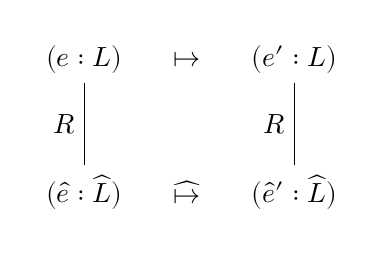
\begin{tikzpicture}[ampersand replacement=\&]

\matrix (m) [matrix of math nodes,row sep=3em,column sep=4em,minimum width=2em]
{ (\Ce : \C) \& (\Ce' : \C) \\
  (\Ae : \A) \& (\Ae' : \A) \\
} ;
\path

(m-1-1) 
edge [white]
node [black] {$\Csteps$} 
(m-1-2)

(m-2-1) 
edge [white]
node [black] {$\Asteps$}
(m-2-2)

(m-1-1) 
edge
node [left] {$R$} 
(m-2-1)

(m-1-2) 
edge
node [left] {$R$} 
(m-2-2)

;

\end{tikzpicture}\end{center}\end{donotbreak}

This picture takes place at some point in the analysis process.
$\Ce$ is the current state (possibly the result of running the original program for a little while).
$\Ae$ is a valid abstraction of $\Ce$, where this validity is expressed by some relation $R$ holding between $\Ce$ and $\Ae$.
$\Ce'$ is some next state of execution of $\Ce$, and likewise for $\Ae$/$\Ae'$.
In order to be a correct analysis, it must be guaranteed that $\Ce'$ and $\Ae'$ will be related.
The logical structure of the picture, which states the correctness of the analysis $\Asteps$, is given by:
\begin{equation*}
∀ (\Ce,\Ce' : \C ) (\Ae,\Ae' : \A), (\Ce R \Ae) ∧ (\Ce \Csteps \Ce') ∧ (\Ae \Asteps \Ae') ⇒  (\Ce' R \Ae')
\end{equation*}
The meaning of the analysis is entirely subject to the relation $R$ which relates the abstract to the concrete.

% }}}

% Galois Connections {{{
\subsection{Galois Connections}
\label{GaloisConnections}

The AI setting can be elegantly simplified and enriched through the use of \emph{Galois connections}.
Galois connections serve as a unifying framework for establishing the “relationship between $\C $ and $\A$” mentioned in the previous section.

A Galois connection between two posets (sets with a partial order) $\C$ and $\A$ is notated $\C\galois{α}{γ}\A$ and contains:
\begin{itemize}
\item $(α : \C → \A)$ where $α$ is monotonic
\item $(γ : \A → \C )$ where $γ$ is monotonic
\item A proof that $(γ ∘ α)$ is expansive: $∀ (x : \C ), x ⊑ γ(α(x))$
\item A proof that $(α ∘ γ)$ is contractive: $∀ (y : \A), α(γ(y)) ⊑ y$
\end{itemize}
The last two properties can be succinctly stated as $(α ∘ γ ⊑ id ⊑ γ ∘ α)$\footnote{
  This uses the usual monotonicity relation $f ⊑ g ⇔  (x ⊑ y ⇒  f(x) ⊑ g(y))$ for the function space.
}.
Equivalent to all four properties is the property $x ⊑ γ(y) ⇔  α(x) ⊑ y$.

A Galois connection $\C\galois{α}{γ}\A$ can be read “$\A$ is an abstraction of $\C$” and $x ⊑ y$ can be read “$x$ is more precise than $y$”.
The expansive property corresponds to \emph{soundness}, and the contractive property corresponds to \emph{tightness}.
A sound analysis gives results you can trust.  
A tight analysis promises to be the “best” analysis possible.

\paragraph{Example:}
Given a Galois connection $\C\galois{α}{γ}\A$, there exists a Galois connection 
  $(\C \xrightarrow{mon} \C)\galois{α'}{γ'}(\A \xrightarrow{mon} \A)$ where:
\begin{align*}
  α'(f : \C \xrightarrow{mon} \C) &≔ α ∘ f ∘ γ \\
  γ'(g : \A \xrightarrow{mon} \A) &≔ γ ∘ g ∘ α \\
\end{align*}

\paragraph{Example:} 
The language $(\PM(ℤ),+,*)$ forms a Galois connection with the language $(\PM(\{ EVEN, ODD \}),∧,∨)$ where:
\begin{align*}
α(zs : \PM(ℤ))               &≔ \{ EVEN  \;|\; ∃ z ∈ zs ∧ Even(z) \} ∪ \{ ODD   \;|\; ∃ z ∈ zs ∧ Odd(z) \}  \\
γ(ts : \PM(\{ EVEN, ODD \})) &≔ \{ z ∈ ℤ \;|\; EVEN ∈ ts ∧ Even(z) \} ∪ \{ z ∈ ℤ \;|\; ODD ∈ ts ∧ Odd(z) \} \\
\end{align*}

Galois connections simplify the AI framework by using $x ⊑ γ(y)$ or (equivalently) $α(x) ⊑ y$ as the relation $(x R y)$.
Galois connections are a natural and general way of placing partial orders \emph{on sets themselves}.
$x ⊑ γ(y)$ can be seen as a heterogenous extension of $x ⊑ y$ when $(x : A)$ and $(y : B)$ live in different sets. 
One can also think of Galois connections as something like an isomorphism, but with a weaker round-trip property.
(An isomorphism would require $α ∘ γ = id = γ ∘ α$.)

Using Galois connections, the AI framework introduced in the previous section can be re-stated. In the AI framework, an analysis for $\Ce$ is:
\begin{itemize}
\item 
  An abstract language $\A$.
\item 
  A Galois connection $\C\galois{α}{γ}\A$.
\item 
  An abstract version of the $\Csteps$ relation: $(\Asteps : \A × \A → Prop)$
\item 
  A way to explore every state reachable by $\Ae$ under $\Asteps$.
  This often requires $\A$ to be finite.
\end{itemize}
The overall approach is summarized in the following picture:
\begin{donotbreak}
\begin{center}
\begin{tabular*}{0.66\textwidth}{@{\extracolsep{\fill}} c c}

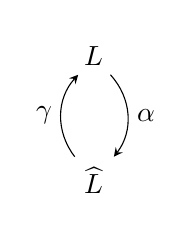
\begin{tikzpicture}[ampersand replacement=\&]
\matrix (m) [matrix of math nodes,row sep=3em,column sep=4em,minimum width=2em]
{ \C \\
  \A \\
} ;
\path [-stealth]

(m-1-1) 
edge [bend left=40]
node [right] {$α$} 
(m-2-1)

(m-2-1) 
edge [bend left=40]
node [left] {$γ$} 
(m-1-1)

;
\end{tikzpicture}

&

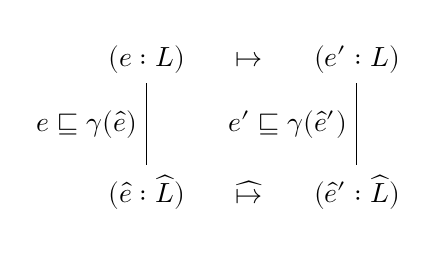
\begin{tikzpicture}[ampersand replacement=\&]
\matrix (m) [matrix of math nodes,row sep=3em,column sep=4em,minimum width=2em]
{ (\Ce : \C) \& (\Ce' : \C) \\
  (\Ae : \A) \& (\Ae' : \A) \\
} ;
\path

(m-1-1) 
edge [white]
node [black] {$\Csteps$} 
(m-1-2)

(m-2-1) 
edge [white]
node [black] {$\Asteps$}
(m-2-2)

(m-1-1) 
edge
node [left] {$\Ce ⊑ γ(\Ae)$} 
(m-2-1)

(m-1-2) 
edge
node [left] {$\Ce' ⊑ γ(\Ae')$} 
(m-2-2)

;
\end{tikzpicture}

\end{tabular*}
\end{center}
\end{donotbreak}

As before, the logical structure of the picture, which states the correctness of the analysis $\Asteps$, is given by:
\begin{equation*}
∀ (\Ce,\Ce' : \C ) (\Ae,\Ae' : \A), (\Ce ⊑ γ(\Ae)) ∧ (\Ce \Csteps \Ce') ∧ (\Ae \Asteps \Ae') ⇒  (\Ce' ⊑ γ(\Ae'))
\end{equation*}
The statement of this property can be simplified further as $\Csteps ⊑ γ(\Asteps)$.
This uses the definition of Galois connections for function spaces shown in a previous example.

Using a Galois connection $\C\galois{α}{γ}\A$ and abstract step function $\Asteps ⊑ γ(\Csteps)$, an algorithm for analysis can be stated:
\begin{enumerate}
\item Translate $(\Ce : \C)$ to $(α(\Ce) : \A)$
\item Explore all abstract states $\Ae'$ states reachable from $α(\Ce)$.
\end{enumerate}
All reachable concrete states are then summarized by projecting each $γ(\Ae')$ back to $\C$.

The Galois connection framework simultaneously justifies the \emph{soundness} and \emph{tightness} of this method.
Soundness tells us that if we (1) abstract, (2) take an abstract step, and then (3) concretize, 
  then the result is an approximation of (4) taking a concrete step.
Soundness tells us that we can trust the results of the analysis.
\begin{donotbreak}
\begin{center}

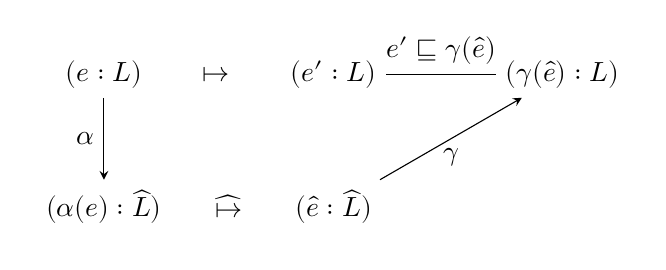
\begin{tikzpicture}[ampersand replacement=\&]
\matrix (m) [matrix of math nodes,row sep=3em,column sep=4em,minimum width=2em]
{ (\Ce : \C)    \& (\Ce' : \C) \& (γ(\Ae) : \C) \\
  (α(\Ce) : \A) \& (\Ae : \A)  \&               \\
} ;
\path [-stealth]

(m-1-1) 
edge
node [left] {$α$} 
(m-2-1)

(m-2-1) 
edge [white]
node [black] {$\Asteps$}
(m-2-2)

(m-2-2)
edge
node [below] {$γ$} 
(m-1-3) 

(m-1-1) 
edge [white]
node [black] {$\Csteps$} 
(m-1-2)

;

\path

(m-1-2)
edge
node [above] {$\Ce' ⊑ γ(\Ae)$}
(m-1-3)

;
\end{tikzpicture}

\end{center}
\end{donotbreak}


Tightness tells us that if we (1) concretize, (2) take a concrete step, and then (3) abstract, 
  then the result must be just as precise as (4) taking an abstract step.
Tightness tells us that our abstract step function isn't losing precision unnecessarily, 
  and that our abstract step $\Asteps$ is provably as precise as possible.
\begin{donotbreak}
\begin{center}

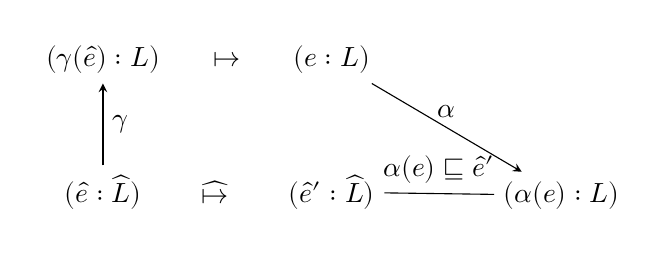
\begin{tikzpicture}[ampersand replacement=\&]
\matrix (m) [matrix of math nodes,row sep=3em,column sep=4em,minimum width=2em]
{ (γ(\Ae) : \C) \& (\Ce : \C) \&                \\
  (\Ae : \A)    \& (\Ae' : \A) \& (α(\Ce) : \C) \\
} ;
\path [-stealth]

(m-2-1) 
edge
node [right] {$γ$} 
(m-1-1)

(m-1-1) 
edge [white]
node [black] {$\Csteps$}
(m-1-2)

(m-1-2)
edge
node [above] {$α$} 
(m-2-3) 

(m-2-1) 
edge [white]
node [black] {$\Asteps$} 
(m-2-2)

;

\path

(m-2-2)
edge
node [above] {$α(\Ce) ⊑ \Ae'$}
(m-2-3)

;
\end{tikzpicture}

\end{center}
\end{donotbreak}



The above diagrams compose to state similar properties about $\Csteps*$ and $\Asteps*$.

% }}}

% Control Flow Analysis {{{
\subsection{Control Flow Analysis}
\label{CFA}

Control flow analysis is a class of analysis which is particularly important for higher-order languages.
In non-higher-order languages, it can be useful to distinguish control-flow from data-flow.
The control flow of the program is the graph of what functions are called from where.
The data flow of a program is the mapping of which values flow to which variables.
Traditionally one performs a control-flow analysis first to find out which functions are called, 
  and a data-flow analysis second using the results of the control flow analysis.
In higher-order languages, data-flow and control-flow are tightly coupled.
Before you can tell which functions will be called, you need to know how values will flow through the program.

We note that the distinction between “higher-order” languages and “non-higher-order” languages is a red herring.
Functions can be passed as values in C using function pointers.
Object-oriented languages enjoy a similar circularity between control and data flow from dynamic method dispatch.
You can read these statements as saying “all languages are higher order, and thus all languages need higher order control flow analysis”.
Or you can read them as saying “all languages are higher order, and we've done just fine without higher oder control flow analysis so far”.
The distinction in practice comes from the properties you are looking for and the code that you end up analysing.

We build on the tradition of Control Flow Analysis (CFA) pioneered by Shivers\cite{shivers:1991:cfa}.
In this tradition, the result of a control flow analysis is closer to what one would think of as a data-flow analysis.
CFA is nothing more than getting data-flow right in a higher-order setting.
0CFA, the most basic control flow analysis, merely computes the set of values which might flow to a particular variable.
kCFA is a family of context sensitive extensions to 0CFA which separates analysis results for functions based on call site.
We use 0CFA and kCFA as the example analyses in this paper.

% }}}

% Monads {{{
\subsection{Monads}
\label{Monads}

Some find it useful to review the concept of functor before learning about monads. 
We adopt this approach for our brief explanation of monads.

\paragraph{Functors}
A type $(F : Set → Set)$ is called a \emph{functor} if one can:
\begin{itemize}
\item Define $map : ∀ (A, B : Set), (A → B) → (F(A) → F(B))$
\item Prove $map(id) = id$
\item Prove $map (g ∘ f) = map(g) ∘ map(f)$
\end{itemize}

\begin{example}
Lists are functors, where $map$ is defined:
\begin{align*}
    map(f)(xs) ≔ &\case(xs):           \\
          Nil    &→ Nil                \\
         x ∷ xs' &→ f(x) ∷ map(f)(xs') \\
\end{align*}
\end{example}

\begin{example} 
  $map(isEven)([1, 2, 3, 4]) = [False, True, False, True]$ 
\end{example}

\paragraph{Monads}
A type $(ℳ  : Set → Set)$ is called a \emph{monad} if one can:
\begin{itemize}
\item Define $extend : ∀ (A, B : Set), (A → ℳ (B)) → (ℳ (A) → ℳ (B))$
\item Prove $extend(return) = id$, called the left-unit law.
\item Prove $extend(f)(return(x)) = f(x)$, called the right-unit law.
\item Prove $extend(g)(extend(f)(x)) = extend(λ(y) → extend(g)(f(y)))(x)$ called associativity.
\end{itemize}
The only computational difference from the definition of functor is in the first argument of extend.
For monads, this argument is allowed to be a \emph{monadic} $(A → ℳ (B))$, rather than a pure function $(A → B)$.

\begin{example} Lists are monads, where $extend$ is defined:
\begin{align*}
    extend(f)(xs) ≔ &\case(xs):                                                                 \\
                Nil &→ Nil                                                                      \\
            x ∷ xs' &→ f(x) ⧺\footnote{⧺ is our notation for list concatenation} extend(f)(xs') \\
\end{align*}
\end{example}

\begin{example} 
Let $adjacent(x) ≔ [x - 1, x + 1]$.  Then $extend(adjacent)([10, 100]) = [9, 11, 99, 101]$
\end{example}

\paragraph{Monad Notation}
One of the biggest benefits of monads is perhaps the most superficial: do-notation.
Do-notation transforms imperative-looking code into uses of $extend$.
This enables kind of “abstract semicolon”, where the meaning of sequencing statements is give by an arbitrary implementation of $extend$.

Do-notation is simply a translation from:
\begin{align*}
  do&                  \\
    &x ← get           \\
    &y ← get           \\
    &put(x + y)        \\
\end{align*}
to
\begin{align*}
  extend(λ(x) → extend(λ(y) → put(x + y)(get)))(get)
\end{align*}

Leveraging even more notation, we can write $extend(f)(x)$ infix and backwards as $x ≫= f$, yielding the following equivalent translation:
\begin{align*}
  &get ≫= λ(x) →    \\
  &get ≫= λ(y) →    \\
  &put(x + y)       \\
\end{align*}
which looks closer to the original expression written in do-notation.
For the rest of the paper we will write exclusively using do-notation and assume this lightweight translation to uses of $extend$.

% }}}

% Monadic Effects {{{
\subsection{Monadic Effects}
\label{MonadicEffects}

In addition to $return$ and $extend$, monads typically come with their own flavor of \emph{monadic effect}.
We use two monadic effects in this paper: state and nondeterminism.

\paragraph{State}
The state monadic effect models manipulation of a single cell of state with type $𝓈$ using operations $get$ and $put$:
\begin{align*}
  get &: ℳ (𝓈)      \\
  put &: 𝓈 → ℳ (1)  \\
\end{align*}
(We write $1$ as the unit type, i.e. the singleton set.)
$get$ and $put$ come with the following laws:
\begin{align*}
               put(𝓈_1) ; put(𝓈_2) &= put (𝓈_2)           \\
                      put(𝓈) ; get &= return(𝓈)           \\
                  𝓈 ← get ; put(𝓈) &= return(∙)           \\
𝓈_1 ← get ; 𝓈_2 ← get ; k(𝓈_1,𝓈_2) &= 𝓈 ← get ; k(𝓈,𝓈)    \\
\end{align*}
Multiple cells of state can be modeled by stacking this effect multiple times.  

\paragraph{Nondeterminism}
The nondeterminism monadic effect models branching control flow using a single operation $⟨+⟩$:
\begin{align*}
    ⊥ &: ∀ (a : A), ℳ (A)                  \\
  ⟨+⟩ &: ∀ (a : A), ℳ (A) → ℳ (A) → ℳ (A)  \\
\end{align*}
$⟨+⟩$ comes with the following laws:
\begin{align*}
         extend(\_)(⊥) &= ⊥                                \\
  extend(const(⊥))(\_) &= ⊥                                \\
    extend(f)(x\; ⟨+⟩\; y) &= extend(f)(x)\; ⟨+⟩\; extend(f)(y)    \\
\end{align*}
A null branch of a computation is written $⊥ $ and branching with two possible values $v_1 v_2$ is written $return(v_1)\; ⟨+⟩\; return(v_2)$.
Note that $ℳ $ having a nondeterminism effect is equivalent to $ℳ $ being a join-semilattice for every possible $ℳ (a)$.

% }}}

% Monad Transformers {{{
\subsection{Monad Transformers}
\label{MonadTransformers}

Monad transformers are building blocks for constructing larger monads.
Where a monad $ℳ $ will have type $Set → Set$, a monad transformer $𝒯$ will have type $(Set → Set) → (Set → Set)$.
Monad transformers are used to extend an existing monad to support another effect.

The three monads used in this work are the state monad, nondeterminism monad, and identity monad.
The state monad is notated $\SM(𝓈)$ (carrying a single cell of type $𝓈$), nondeterminism $\PM$, and identity $ID$.
The transformer analogues for state and nondeterminism are notated $\ST(𝓈)(ℳ )$ and $\PT(ℳ )$ where $ℳ $ is the underlying monad.
The transformer versions of both of these monads allow you to combine effects piecewise.

\begin{example}
  $\ST(ℤ)(\PT(ID))$ and $\PT(\ST(ℤ)(ID))$ are both monads with state (where $𝓈 = ℤ$) and nondeterminism effects.
\end{example}

The non-transformer versions of state and nondeterminism monads can be defined directly, or simply as transformers on top of $ID$.
The nondeterminism monad transformer we use in this work is new.
The full definitions and proofs of all monad transformers used in this paper are given in section \ref{Proofs}.

% }}}

% }}}

% A Compositional Analysis Framework {{{

\section{A Compositional Analysis Framework}
\label{CompositionalAnalysis}

A compositional analysis framework must support adding and removing features from the analysis without touching the entire implementation.
We achieve such compositionality by building abstract interpreters using monad transformers.
To demonstrating our compositional approach to analysis design, we first show a classic definition of 0CFA.
Then, we will show how to design such an analysis using our framework.
After porting 0CFA to our framework, we will show how to grow this analysis to include context sensitivity in a compositional fashion.

We will use the CPS-IF language introduced in section \ref{CPS} as the target language for 0CFA.
We repeat the definition of CPS-IF syntax here for convenience.
\begin{align*}
x,y,k : Var  &⩴ ...variables...                                          \\
b,i,l : Lit  &⩴ ℤ ∪ 𝔹                                                    \\
  f,g : Lam  &⩴ \lam(x) → e \;|\; \lam(x,k) → e                          \\
    a : Atom &⩴ x \;|\; l \;|\; f \;|\; op(a)                            \\
   op : Op   &⩴ \add \;|\; \sub \;|\; \gez                               \\
    e : Exp  &⩴ \iif(a)\{e\}\{e\} \;|\; a(a) \;|\; a(a,a) \;|\; \halt(a) \\
\end{align*}



\subsection{Classic 0CFA}
\label{AAM-0CFA}

Our abstract semantics for classic 0CFA will track literals (including lambdas) that appear in the program text.
For integers that do not appear in the program text, the analysis uses a single token $INT$ which conservatively approximates any possible integer.
We note that many more abstractions for integers are possible, like integer ranges or symbolic binary relations among variables.
These decisions do not interfere with AAM or abstract control, so we pick the simplest abstraction to simplify presentation.

The state space $\A$ for 0CFA is defined as:
\begin{align*}
v : \AVal   &⩴ l \;|\; f \;|\; INT \;\;(\text{where $l$ and $f$ are drawn from the program text}) \\
θ : \AStore &≔ Var → \PM(\AVal)                                                               \\
\Ae : \A    &≔ \PM(Exp × \AStore)                                                             \\
\end{align*}

Because there are finite many literals in the program text, we can claim that $\AVal$ and $\AStore$ are finite.

The abstract semantics for $\A$ comes in two parts.  
First we define a \emph{denotation function} $𝒜 $ for $Atom$ expressions.
\begin{align*}
𝒜                    &: \AStore × Atom → \PM(\AVal)                 \\
𝒜 (θ,x)              &≔ θ(x)                                        \\
𝒜 (θ,l)              &≔ \{ l \}                                     \\
𝒜 (θ,\add(a))         &≔ \{ \INT \;|\; ∃ i ⊑ \INT ∈ 𝒜 ( θ , a) \}    \\
𝒜 (θ,\sub(a))         &≔ \{ \INT \;|\; ∃ i ⊑ \INT ∈ 𝒜 ( θ , a) \}    \\
𝒜 (θ,\gez(a))         &≔ \{ \TRUE \;|\; ∃ i ∈ 𝒜 (θ,a) ∧ i >= 0 \}    \\
                     &∪ \{ \FALSE \;|\; ∃ i ∈ 𝒜 (θ,a) ∧ i < 0 \}    \\
                     &∪ \{ \TRUE, \FALSE \;|\; \INT ∈ 𝒜 ( θ , a) \} \\
𝒜 (θ,\lam(x) → e)    &≔ \{ \lam(x) → e \}                           \\
𝒜 (θ,\lam(x)(k) → e) &≔ \{ \lam(x)(k) → e \}                        \\
\end{align*}



Second we define a \emph{step relation} (as a function) $ℰ$ for $Exp$ expressions.
\begin{align*}
ℰ                        : &Exp × \AStore → \PM(Exp × \AStore)                                       \\
ℰ(\iif(a)\{e₁\}\{e₂\},θ) ≔ &\{ (e,θ)                                                                 \\
                           &|\; e ∈ \{ e₁ \;|\; \TRUE ∈ 𝒜 (θ,a) \} ∪ \{ e₂ \;|\; \FALSE ∈ 𝒜 (θ,a) \} \\
                           &\}                                                                       \\
          ℰ(a₁(a₂,a₃),θ) ≔ &\{ (e,θ')                                                                \\
                           &|\; (\lam(x)(k) → e) ∈ 𝒜 (θ,a₁)                                          \\
                           &|\;             v₂ ∈ 𝒜 (θ,a₂)                                            \\
                           &|\;             v₃ ∈ 𝒜 (θ,a₃)                                            \\
                           &|\;             θ' ≔ θ ⊔ [x ↦ v₂] ⊔ [k ↦ v₃]                             \\
                           &\}                                                                       \\
           ℰ(\halt(a),θ) ≔ &\{ (\halt(a),θ) \}                                                       \\
\end{align*}

(We omit the $(a₁(a₂))$ case. It is directly analogous to $(a₁(a₂,a₃))$).

The complete analysis of an expression $e$ is defined as the least fixed point of a \emph{collection semantics} for the relation $ℰ$:
\begin{align*}
\text{analysis} ≔ μ(\Ae) → \{(e,⊥)\} ⊔ ℰ^{⋆}(\Ae)
\end{align*}
where
\begin{align*}
ℰ^{⋆}    &: \PM(Exp × \AStore) → \PM(Exp × \AStore) \\
  ℰ^{⋆}(\Ae) &≔ ⋃_{e, θ ∈ \AE} ℰ(e,θ) \\
\end{align*}
A collecting semantics is used to track all states that the program could be in rather than just the final states.

\subsection{Monadic 0CFA}
\label{MAAM-0CFA}

The first insight in monadic abstract interpretation is to abbreviate the definitions of $𝒜 $ and $ℰ$ using monadic state.
We use a nondeterminism monad underneath a state monad transformer to write the analysis in monadic style.
Monad transformers are just fancy names for simple types, 
  and we write simple types underneath definitions which use monad transformer to aid understanding.
\begin{align*}
ℳ     &: Set → Set                  \\
ℳ (a) &≔ \ST(\AStore)(\PM)(a)       \\
ℳ (a) &≔ \AStore → \PM(a × \AStore) \\
\end{align*}


The monadic conversion of $𝒜 $ interacts with the store $θ$ using get and put operations.
\begin{align*}
𝒜_{m}                 &: Atom → ℳ (\PM(\AVal))                         \\
𝒜_{m}(x)              &≔ \ddo                                          \\
                      &θ ← \getstore                                   \\
                      &\return(θ(x))                                   \\
𝒜_{m}(l)              &≔ \return(\{l\})                                \\
𝒜_{m}(add1(a))        &≔ \ddo                                          \\
                      &v ← 𝒜_{m}(a)                                    \\
                      &\return(\{\INT \;|\; ∃ i ⊑ \INT ∈ v\})          \\
𝒜_{m}(sub1(a))        &≔ \ddo                                          \\
                      &v ← 𝒜_{m}(a)                                    \\
                      &\return(\{\INT \;|\; ∃ i ⊑ \INT ∈ v\})          \\
𝒜_{m}(gez(a))         &≔ \ddo                                          \\
                      &v ← 𝒜_{m}(a)                                    \\
                      &return(\{ \TRUE \;|\; ∃ i ∈ v ∧ i >= 0 \} ∪ \{ \FALSE \;|\; ∃ i ∈ v ∧ i < 0 \} ∪ \{ \TRUE, \FALSE \;|\; INT ∈ v \}) \\
𝒜_{m}(\lam(x)(k) → e) &≔ \return(\{\lam(x)(k) → e\})                   \\
\end{align*}


The monadic conversion of $ℰ$ uses $\liftpowerset$ to convert from powerset to monadic values.
$\coercebool$ and $\coercefun$ are used to coerce lambdas out of abstract values, failing (with $⊥$) otherwise.
The “effects” in $ℰ_{m}$ happen in calls to $𝒜_{m}$, $\liftpowerset$, $\coercebool$ and $\coercefun$.
\begin{align*}
                     ℰ_{m} &: Exp → ℳ (Exp)                                                    \\
ℰ_{m}(\iif(a)\{e₁\}\{e₂\}) &≔ \ddo                                                             \\
                           &vP ← 𝒜_{m}(a)                                                      \\
                           &v ← \liftpowerset(vP)                                              \\
                           &b ← \coercebool(v)                                                 \\
                           &\return(\{ \text{if}\; b\; \text{then}\; e₁\; \text{else}\; e₂ \}) \\
          ℰ_{m}(a₁(a₂,a₃)) &≔ \ddo                                                             \\
                           &vP ← 𝒜_{m}(a₁)                                                     \\
                           &v ← \liftpowerset(vP)                                              \\
                           &(\lam(x)(k) → e) ← \coercefun(v)                                   \\
                           &vP₂ ← 𝒜_{m}(a₂)                                                    \\
                           &vP₃ ← 𝒜_{m}(a₃)                                                    \\
                           &θ ← \getstore                                                      \\
                           &\putstore(θ ⊔ [x ↦ vP₂] ⊔ [k ↦ vP₃])                               \\
                           &\return(e)                                                         \\
\end{align*}


$\liftpowerset$, $\coercebool$ and $\coercefun$ use the nondeterminism monadic effect and are defined as follows:
\begin{align*}
                 \liftpowerset &: 𝒫 (a) → ℳ (a)                        \\
\liftpowerset(\{x₁, ..., x₂\}) &≔ ⋃ \{return (x₁), ... , return (x₂)\} \\
                                                                       \\
                   \coercebool &: \AVal → ℳ  (𝔹 )                      \\
               \coercebool (b) &≔ return(b)                            \\
              \coercebool (\_) &≔ ⊥                                    \\
                                                                       \\
                    \coercefun &: \AVal → ℳ  (Lam)                     \\
                \coercefun (f) &≔ return(f)                            \\
               \coercefun (\_) &≔ ⊥                                    \\
\end{align*}


The monadic abstraction leads to a more compositional definition of the analysis.
Pieces of the analysis which only use one effect need not mention the others.
This compositionality will become more apparent when we extend this analysis to include context sensitivity.

As before, we must complete the analysis by building an abstract machine transition function:
\begin{align*}
ℰ_{m}^{⋆}    &: \PM(Exp × \AStore) → \PM(Exp × \AStore) \\
  ℰ_{m}^{⋆}(\Ae) &≔ ⋃_{e, θ ∈ \Ae} ℰ_{m}(e)(θ) \\
\end{align*}
This definition of $ℳ $ and $ ℰ_{m}^{⋆}$ recovers exactly the analysis we wrote before.

\subsection{Monadic kCFA}
\label{MAAM-kCFA}

To incorporate context sensitivity (for $k=1$) into the analysis we do the following:
\begin{itemize}
\item Add another state space component to $\A$ for environments: $\AEnv$.
      This environment will track which calling function is responsible for binding a given parameter.
\item Capture this environment when evaluating $λ$ expressions, just the concrete semantics does for concrete environments.
\item Add another state space component which tracks the program points visited so far by the program: $\ATime$.
\item When interpreting a command $ℰ_{m}(e)$ set the time to $e$.
\item When calling a function, record the current time next to the function arguments in the environment.
\end{itemize}
These steps have the effect of re-analyzing a function twice if it is called from two separate places.

Changing the state space two have two new components is achieved simply by adding two more state effects two our monad, 
  one for $\AEnv$ and one for $\ATime$.
The resulting abstract state space looks like this:
\begin{align*}
  ρ : \AEnv &≔ Var ⇀ \ATime                                     \\
θ : \AStore &≔ (Var,\ATime) → \PM(\AVal)                        \\
 τ : \ATime &≔ Exp \;\text{(the last program location visited)} \\
 f,g : Lam  &⩴ \lam(x) → e \;|\; \lam(x,k) → e                  \\
  clo : Clo &⩴ ⟨f, ρ⟩                                           \\
  v : \AVal &⩴ l \;|\; clo \;|\; INT                            \\
  \Ae : \A  &≔ \PM(Exp × \ATime × \AEnv × \AStore)              \\
\end{align*}

Using monad transformers, we can easily add two new state components to our monadic interpreter.
\begin{align*}
ℳ     &: Set → Set                                                    \\
  ℳ (a) &≔ \ST(\AEnv)(\ST(\ATime)(\ST(\AStore)(\PM))(a)               \\
ℳ (a) &≔ \AEnv × \ATime × \AStore → \PM(a × \AEnv × \ATime × \AStore) \\
\end{align*}

Capturing the environment when evaluating $λ$ expressions is a simple use of monadic state:
\begin{align*}
𝒜_{m}                &: Atom → ℳ (\PM(\AVal)) \\
                 ... &                        \\
𝒜_{m}(f)             &≔ \ddo                  \\
                     &ρ ← \getenv             \\
                     &\return (\{⟨f, ρ⟩\})    \\
                 ... &                        \\
\end{align*}

Moving abstract time forward is a simple update of the $\ATime$ state to be the current expression:
\begin{align*}
   ℰ_{m}' &: Exp → ℳ (Exp) \\
ℰ_{m}'(e) &≔ \ddo          \\
          &\puttime(e)     \\
          &ℰ_{m}(e)        \\
\end{align*}

Calling a function now uses time as an address for storing values in $\AStore$.
This is analogous to the allocation concrete semantics shown in section \ref{CPS}.
\begin{align*}
           ℰ_{m} &: Exp → ℳ (Exp)                              \\
             ... &                                             \\
ℰ_{m}(a₁(a₂,a₃)) &≔ \ddo                                       \\
                 &vP ← 𝒜_{m}(a₁)                               \\
                 &v ← \liftpowerset(vP)                        \\
                 &(⟨\lam(x)(k) → e, ρ⟩) ← \coercefun(v)        \\
                 &vP₂ ← 𝒜_{m}(a₂)                              \\
                 &vP₃ ← 𝒜_{m}(a₃)                              \\
                 &θ ← \getstore                                \\
                 &τ ← \gettime                                 \\
                 &\putenv(ρ[x ↦ τ][k ↦ τ])                     \\
                 &\putstore(θ ⊔ [(x,τ) ↦ vP₂] ⊔ [(k,τ) ↦ vP₃]) \\
                 &\return(e)                                   \\
             ... &                                             \\
\end{align*}

Finally, lookup for variables must follow the indirection of addresses through $\AStore$.
\begin{align*}
𝒜_{m}                &: Atom → ℳ (\PM(\AVal)) \\
                 ... &                        \\
𝒜_{m}(x)             &≔ \ddo                  \\
                     &ρ ← \getenv             \\
                     &θ ← \getstore           \\
                     &\return (θ(x,ρ(x)))     \\
                 ... &                        \\
\end{align*}

That's all there is to it.  
Adding two new states to the state space and instrumenting the analysis to track time leaves the rest of the semantics undisturbed.
Without the monad abstraction, the entire semantics must be redefined when extending the analysis to be context sensitive.

So far we have used monad transformers to build analyses in a compositional manner.
In the next section, we will see how to exploit the monadic abstraction to expose a tuning knob for abstract control.

% }}}

% Abstract Control {{{
\section{Abstract Control}
\label{AbstractControl}

The instantiation for $ℳ $ in our previous examples happens to give a flow-sensitive path-sensitive analysis.
We claim that our monad transformers compose in either direction, 
  and one might ask what happens when one swaps the order of state and nondeterminism transformers.
Consider such a reordering of $ℳ $ (using the simpler 0CFA semantics):
\begin{align*}
ℳ     &: Set → Set                  \\
ℳ (a) &≔ \PT(\SM(\AStore))(a)       \\
ℳ (a) &≔ \AStore → \PM(a) × \AStore \\
\end{align*}

The implementations of $𝒜 $ and $ℰ$ can be left as is, as they did not depend on the specific monad used, only the monadic effect interface.
However, the type of $ℳ $ has changed so we must redefine $ℰ_{m}^{⋆}$, as the old one is now ill-typed.
One possible definition for $ ℰ_{m}^{⋆}$ is the following:
\begin{align*}
ℰ_{m}^{⋆}       &: \PM(Exp) × \AStore → \PM(Exp) × \AStore                                       \\
  ℰ_{m}^{⋆}(eP,θ) &≔ (\{ e' \;|\; e' ∈ π₁(ℰ_{m}(e))(θ) \;\;|\;\; e ∈ e\PM \}, ⋃_{e ∈ eP} π₂(ℰ(e))(θ)) \\
\end{align*}
This definition gives a flow-insensitive path-insensitive analysis.
Note that the resulting state space $\A = \PM(Exp) × \AStore$.

Another implementation of $ℰ_{m}^{⋆}$ is actually possible for a different state space $\A = \PM(Exp × \AStore)$.
This is the same $\A$ from our first monadic definition of 0CFA, although we are using a different monad.
\begin{align*}
ℰ_{m}^{⋆}    &: \PM(Exp × \AStore) → \PM(Exp × \AStore)                             \\
ℰ_{m}^{⋆}(\Ae) &≔ \{ (e',π₂(ℰ_{m}(e))(θ)) \;\;|\;\; e' ∈ π₁(ℰ_{m}(e))(θ) \;\;|\;\; (e,θ) ∈ \Ae \} \\
\end{align*}
This definition gives a flow-sensitive path-insensitive analysis.

By altering the monad behind the abstraction, we are able to tune the flow and path sensitivity of the analysis.
The two choices for $ℳ $ alter to path sensitivity of the analysis.
For the choice of $ℳ  = \PT(\SM(\AStore))$, the two choices for $\A$ alter the flow sensitivity of the analysis.

Our definition of a nondeterminism monad transformer is new in this work, and we give its definition here.
Our nondeterminism monad transformer requires the underlying monad $ℳ $ to be a join-semilattice functor: 
  $ℳ (a)$ must be a join-semilattice if $a$ is a join-semilattice.
We define the type $\PT(ℳ )(a) ≔ ℳ (\PM(a))$ and define monad operations:
\begin{align*}
   return &≔ return_{ℳ } ∘ singleton \\
extend(k) &≔ extend_{ℳ }(joins ∘ map_{\PM}(k))  \\
\end{align*}
where
\begin{align*}
  joins(xs) ≔ ⋃_{x ∈ xs} x
\end{align*}
The fact that $\PT(ℳ )(a)$ is a join-semilattice follows trivially from the functorality of $ℳ $.
Proofs of monad laws and other correctness properties are given in section \ref{Proofs}.

% }}}

% Intensional Optimizations {{{
\section{Intensional Optimizations}
\label{Optimizations}

Up to this point we have demonstrated a compositional framework for building abstract interpreters, 
  and a method for exposing abstract control as a tuning knob for these analysis.
Now we show how to implement two intentional optimizations, abstract garbage collection and MCFA, in a completely general setting.

\subsection{Abstract Garbage Collection}
Abstract garbage collection\cite{might:2006:gammacfa} is an optimization technique in abstract interpretation 
  where unreachable abstract addresses are pruned from the state space.
This is analagous to “real” garbage collection, where unreachable pointers are reclaimed for space efficiency.
However, in abstract semantics, live addresses are \emph{re-used} as part of the sound and finite approximation of an infinite address space.
When an in-use address must be re-used for allocation, a static analysis is forced to lose precision.
Abstract garbage collection exploits the fact that unreachable addresses can be reclaimed before they are re-used, 
  resulting in no loss of precision when re-using an address.

For a generic implementation of garbage collection we assume an arbitrary $ℳ $ that has $get$, $put$ and nondeterminism effects.
This allows us to change $ℳ $, and therefore the flow and path sensitivity of the garbage collection, 
  without having to reimplement our optimization.

We implement abstract garbage collection for our example of kCFA (for $k=1$) described in section \ref{MAAM-KCFA}.
Our implementation of garbage collection uses two helper functions $𝓉Exp : Exp → ℳ (\PM(\AAddr))$ and $ 𝓉\AAddr : \AStore → \AAddr → \PM(\AAddr)$.
$𝓉Exp$ is a monadic action which computes the live addresses reachable from the current expression using $ 𝓉\AAddr$.
$𝓉\AAddr$ computes the addresses reachable from a single address.
\begin{align*}
          𝓉Clo &: \AStore × Clo → \PM (\AAddr)         \\
𝓉Clo(θ,⟨f, ρ⟩) &≔ ⋃_{x ∈ freevars(f)} 𝓉\AAddr(θ)(ρ(x)) \\
        𝓉Addr &: \AStore → \AAddr → \AAddr            \\
𝓉\AAddr(θ)(𝓁)  &≔ ⋃_{clo ∈ θ(𝓁)} 𝓉Clo(clo)             \\
       currClo &: Exp → ℳ (Clo)                        \\
  currClo(e)   &≔ \ddo                                 \\
               &ρ ← \getenv                            \\
               &return(⟨λ(\_) → e, ρ⟩)                 \\
          𝓉Exp &: Exp → ℳ (\AAddr)                     \\
  𝓉Exp(e)      &≔ \ddo                                 \\
               &clo ← currClo(e)                       \\
               &𝓉Clo(clo)                              \\
\end{align*}
$freevars$ computes the free variables of an expression in the usual way:
\begin{align*}
  freevars(\iif(a)\{e₁\}\{e₂\}) &≔ freevars(a) ∪ freevars(e₁) ∪ freevars(e₂)   \\
  freevars(a₁(a₂))        &≔ freevars(a₁) ∪ freevars(a₂)                 \\
  freevars(a₁(a₂,a₃))     &≔ freevars(a₁) ∪ freevars(a₂) ∪ freevars (a₃) \\
  freevars(\halt(a))      &≔ freevars(a)                                 \\
  freevars(\lam(x) → e)   &≔ freevars(e) - \{ x \}                       \\
  freevars(\lam(x,k) → e) &≔ freevars(e) - \{ x, k \}                    \\
  freevars(l)             &≔ \{\}                                        \\
\end{align*}

Using helper functions $𝓉Exp$ and $ 𝓉\AAddr$, we can define garbage collection using the following strategy:
\begin{enumerate}
\item Find the set of addresses reachable from the current expression.
\item Find the least-fixed point of the reachability relation for the heap starting from this set.
\item Retain only the mappings in the heap that have keys in this set.
\end{enumerate}
\begin{align*}
   gc &: Exp → ℳ (1)                                     \\
gc(e) &≔ \ddo                                            \\
      &θ ← \getstore                                     \\
      &𝓁₀ ← \touchedexp(e)                              \\
      &\llet 𝓁_{∞} ≔ μ(𝓁) → 𝓁₀ ⊔ 𝓁 ⊔ \touchedvar(𝓁) \\
      &\putstore(⋃_{x ∈ 𝓁_{∞}} [x ↦ (θ(x))])            \\
\end{align*}

This is literally the implementation of \emph{concrete} garbage collection, but with control properties abstracted behind a monad.
When instantiated with path-sensitive, flow-sensitive or flow insensitive monads, 
  we can recover the appropriate version of control for abstract garbage collection.

In AAM, the authors describe abstract garbage collection for a path-sensitive CESK* machine.
Later in the AAM story, the path-sensitive CESK* machine is abstracted to use a single global store, 
  resulting in a less precise but more tractable analysis.
However, the single-store variant of the analysis requires one to repeat the 
  “instrument then abstract” design process all over again for abstract garbage collection.
By abstracting control and exposing it as an orthogonal tuning knob, 
  we are able to design flow and path sensitive variants of garbage collection with a single definition.

\subsection{MCFA}

MCFA\cite{might:2010:mcfa} is an optimization that improves the asymptotic 
  complexity of context-sensitive control flow analyses for functional languages.
Context sensitive analysis were shown to be exponential for functional analyses, yet polynomial for OO analysis, creating an apparent paradox.
MCFA resolves this paradox by identifying the difference in context sensitive analyses and porting the polynomial behavior from OO to functional analyses.
The key insight of MCFA is to use packed, copied closures rather than linked closures in the abstract semantics.
Like garbage collection, using packed rather than linked closures is a simple optimization a compiler or concrete interpreter might use to increase performance.
Like \emph{abstract} garbage collection, transporting this simple idea from concrete to abstract interpreters reveals a surprising analysis optimization.

Like abstract garbage collection, our implementation of MCFA also uses the semantics for kCFA.
MCFA is implemented by creating a new packed environment, rather than just linking with the current environment:
This reuses the definition of $freevars$ from the previous section.
\begin{align*}
𝒜_{m}                &: Atom → ℳ (\PM(\AVal)) \\
                 ... &                        \\
𝒜_{m}(f)             &≔ \ddo                  \\
                     &\llet ys ≔ \operatorname{free-vars}(f)        \\
                     &vs ← map^{⋆}(lookup)(ys)                      \\
                     &ρ ← \{ y ↦^{⋆} v \;|\; (y,v) ∈ zip(ys, vs) \} \\
                     &\return(⟨f,ρ⟩)                                \\
                 ... &                        \\
\end{align*}


Like abstract garbage collection, our implementation of MCFA is tunable from one implementation which has abstracted control through a monad.
Flow and path sensitive variants of MCFA fall out of a simple rearranging of the monad transformer stack.

% }}}

% Correctness {{{
\section{Correctness}
\label{Correctness}

One advantage of using our framework is that proofs of correctness for analyses are constructed compositionally and automatically.
The proofs are compositional because they are established at the level of monad transformers, not hard-coded for a full monad stack.
The proofs are derived automatically through the Galois-functorality of the monad transformers we use, 
  which means they transport Galois connections in addition to monadic actions.
Given the proofs provided by our framework, along with an argument about monotonicity of the monadic semantics, 
  we can establish a proof of Galois connection for any given monadic instantiation.

To relate back to state machine semantics, we establish Galois connections between monadic actions in $ℳ $ 
and transitions functions for \emph{some} abstract state space $\A$, notated $(A \xrightarrow{mon} ℳ (B))\galois{α}{\gamma}(\A_T(A) \xrightarrow{mon} \A_T(B))$.
The abstract state space $\A$is constructed from the monad transformer stack, although some transformer stacks support multiple abstract state spaces.
Proofs of these properties are given in section \ref{Proofs}.

Key lemmas in our construction of these Galois connections include:
\begin{itemize}
\item Proving that our new monad transformer for nondeterminism is a proper monad transformer.
      The key insight here is to require the underlying monad to be a join-semilattice functor, 
         which holds for the analyses we discuss in this paper.
\item Proving that both state and nondeterminism transformers transport Galois connections to abstract state machines.
  The key insight here is to move the Galois connection framework to a \emph{functorial} framework, 
    where $α(1) = 1$ and $ α(g ∘ f) = α(g) ∘ α(f)$, and likewise for $γ$.
\end{itemize}

In our framework we also prove that $(\ST(𝓈) ∘ \PT) ⊑ (\PT ∘ \ST(𝓈))$.
These orders for the monad transformer stack correspond to path-sensitivity and path-insensitivity respectively.

For the $\PT ∘ \ST(𝓈)$ ordering, we show two Galois connections are possible: 
  one to the state space $\PM(\_ × 𝓈)$ and one to the state space $(\PM(\_) × 𝓈)$.
These choices for Galois connection correspond to flow-sensitivity and flow-insensitivity respectively.

Using monad transformers and their relationships to state machines, we have shown independent of a particular language or analysis that:
\begin{align*}
  \text{flow-insensitive} ⊑ \text{flow-sensitive path-insensitive} ⊑ \text{flow-sensitive}
\end{align*}

A given \emph{concrete} semantics will typically use the flow-sensitive path-sensitive monad.
Using this already established ordering we can construct a Galois connection between 
  a concrete semantics and a flow-insensitive abstract semantics with no additional effort.

This table summarizes our results, showing both the monad $ℳ $ and state space $\A$ which correspond to each analysis:
\begin{center}\begin{tabular}{| c | c | c |}
  \hline Sensitivity      & Path Sensitive                             & Path Insensitive                           \\
  \hline Flow Sensitive   & $ℳ  ≔ \ST ∘ \PT$ \;|\; $\A ≔ \PT ∘ \XT$ & $ℳ  ≔ \PT ∘ \ST$ \;|\; $\A ≔ \PT ∘ \XT$ \\
  \hline Flow Insensitive & $DNE$                                      & $ℳ  ≔ \XT ∘ \PT$ \;|\; $\A ≔ \XT ∘ \PT$ \\
  \hline
\end{tabular}\end{center}
where $\XT$ is the state machine functor for cartesian product ($×$).

% }}}

% Related Work {{{
\section{Related Work}
\label{RelatedWork}

\paragraph{Abstract Control}
Johnson and Van Horn recently explored the concept of abstract control in their recent paper Abstracting Abstract Control 
(AAC)\cite{johnson:2014:AAC}.
In this work, the authors discuss how to recover a pushdown abstraction systematically in the setting of AAM.
Our work is orthogonal, and potentially compatible with theirs: our framework explains compositional analyses, while theirs explains pushdown control abstraction.
We hope for an eventual combination of the two techniques, which would expose pushdown abstraction as a feature-independent tuning knob.

As far as the question “what is abstract control?”, we paint a similar picture as do Johnson and Van Horn in AAC.
In both works, abstract control is an abstraction over the fixpoint iteration of the semantic step function which classic AAM didn't account for.
Our work gives one possible definition for what abstract control is: 
  abstrct control is the combination of control effects used by an interpreter,
  coupled with the way these effects are related to abstract machines.

\paragraph{Compositional Approaches}
Another compositional approach to abstract interpretation is \emph{calculational abstract interpretation}\cite{cousot:1999:calculational} 
  as described by Cousot and Cousot.
Calculational AI shares a similar philosophy to our work: abstract interpreters should be built piecewise from compositional components.
In calculational AI, analyses are derived by applying a sequence of Galois connections to the concrete semantics.
This contrasts to the approach of designing an analysis first, and manually justifying the Galois connection after.
However, after applying a sequence of Galois connections, 
  the analysis designer must \emph{calculate} the computable analysis from the one derived by Galois connection composition,
  which in general is not computable.

The downfall of calculational AI is in the effort required during the calculation step.
For example, Midgaard and Jensen\cite{midtgaard:2008:calculational-cfa} describe a calculational derivation of 0CFA, the same analysis described in this work, and it is a difficult process.

While work in calculational AI has perhaps seen less success than AAM, 
  we note that the two approaches are actually compatible, tackling different parts of the analysis design process.
AAM is a methodology for splitting the design process to first instrument a concrete semantics, and then systematically abstract.
Both of these steps must be justified with Galois connections, and one could use calculation for either step.
Our work provides computations and proofs for the abstraction step, but one might happily justify the instrumentation step via calculation.

\paragraph{Tuning Knobs}
Tuning knobs for static analysis are great when they're general enough for a wide range of applications.
For example, work by Kastrinis and Smaragdakis\cite{kastrinis:2013:hybrid-points-to}\cite{smaragdakis:2011:pick-your-contexts-well} 
  shows how to expose both context-sensitivity and object-sensitivity as orthogonal tuning knobs in an OO analysis.
These knobs have shown to be sufficient for interesting applications like malware detection for Android applications\cite{feng:2014:apposcopy}.
(\cite{feng:2014:apposcopy} directly uses the analysis framework described in\cite{kastrinis:2013:hybrid-points-to}.)

\paragraph{Path Sensitivity}
Path sensitivity in particular was shown to be profitible and tractable by Das et al.\cite{das:2002:esp}.
In this work the authors verify the absence of open/close file handle bugs in the GNU C compiler.
Path sensitivity was crucial achieve the precision needed for their analysis, and their paper describes how to achieve this precision without too much added cost in complexity.
These subtle variants of path sensitivity are important for applying path sensitive analysis in practice.
We do not directly account for these particular variants of path sensitivity in our framework, 
  although we hope to explore how they fit into our framework in future work.
% }}}

% Future Work {{{
\section{Future Work}
\label{FutureWork}

\paragraph{Fully Verified Compilation}
One direction of future work is to apply our approach to fully verified compilation.
In fully verified compilation, the implementation of a comipler is typically embedded in proof assistant and proven correct all the way down to axioms in a logical system.
This task is difficult due to both the extra rigor required in modeling and the proof engineering required in interacting with proof assistants.
We hope the compositionality of the \emph{correctness} of our approach will apply especially in this setting, because proofs need to be developed and maintained side-by-side with code.

CompCert\cite{leroy:2009:compcert} is perhaps the most well known fully verified compiler to date.
CompCert compiles C programs down to machine code and performs simple local optimizations.
A variation of CompCert which would support richer language features might benefit from our approach.
Whole program analysis has also not been studied yet in the context of fully verified compilation, 
  perhaps because establishing the proof of correctness is too burdensome.
We hope our technique can be applied to a fully verified compiler for functional program which also performs advanced whole program analysis.

In the author's view, the biggest obstacle to implementing verified static analyses is 
  the difficulty in establishing Galois connections using proof assistants.
Galois connections sit in the middle-ground between computable functions (like an isomorphism) 
  and mere specification (like a characteristic function).
Arguments using Galois connections often start with some infinite set, after which calculation brings the 
  result to something finite and computable.
It is this process, moving from infinite to computable through calculation, that we conjecture has given experts the most difficulty in modeling Galois connections.
All results to date of static analyses proven correct within proof assistants give up on establishing full Galois connection 
  and settle for more direct methods.
Tackling this problem could be a huge step forward in bringing more powerful analyses to the stage of fully verified compilation.

\paragraph{New Tuning Knobs for Analysis}
Another direction for future work is to discover more tuning knobs for analyses which have been missed by frameworks like AAM.
For example, it would be nice if we could account for the pushdown abstraction 
  from Johnson and Van Horn's work on Abstracting Abstract Control into our monadic formulation.

Less related to abstract control, we believe there is work to be done in porting object sensitivity to functional language analysis.
We have preliminary results suggesting that object sensitivity can be seen as lexically scoped time in the functional setting.
Exploring this would uncover yet another tuning knob to analysis designers to quickly interate through the analysis design process.

\paragraph{New Semantic Settings}
Our framework shares the small-step operational semantics roots of AAM.
The small-step setting is convenient, but understood consequences when used as the basis for abstract interpretation 
  which are less well understood.

For example, we can imagine a more denotational variant of this work where interpreters are related to a denotational space 
  rather than to state machines.
We have preliminary results suggesting that this can be done by allowing the monadic interpreter to be recursive, 
  and then abstracting the meaning of recursion directly.
The meaning of a program would then be given not given by an external fixpoint of the step function, 
  but directly through a denotation for recursion.
To recover an analysis, one would abstract a precise fixpoint finder like the Y-combinator with an approximating, finite fixpoint finder.

% }}}

% Conclusion {{{
\section{Conclusion}
\label{Conclusion}

We have shown how to build compositional abstract interpreters which expose a tuning knob for abstract control.
We use monad transformers as the building blocks for both constructing abstract interpreters and proving them correct piecewise.
Using the monadic abstraction, we showed how to expose abstract control as a tuning knob to recover flow and path sensitivities 
  for a static analysis.
After exposing a tuning knob for abstract control, we then demonstrated how to implement two analysis optimizations which adapt effortlessly to changes in abstract control.
Our approach is justified piecewise by relating monad transformers to state machine functors.
To achieve this, we develop a new monad transformer for nondeterminism and develop a functorial variant of Galois connection.

When using our framework, the analysis designer need only prove prove:
\begin{itemize}
\item The monadic interpreter $ℰ_{m}$ is monotonic.
\item The semantics as written, including intensional optimizations, are correct.
\end{itemize}
After supplying these proofs, the analysis designer enjoys:
\begin{itemize}
\item An automatically derived analysis for their language with abstract control left as a tuning knob.
\item A proof-by-construction of Galois connection (soundness and tightness) for the derived analysis.
\item Easy integration of new analysis features, a la. AAM.
\item Single-definition implementations of intensional optimizations like abstract garbage collection and MCFA.
\end{itemize}

% }}}

% Proofs {{{
\section{Proofs}
\label{Proofs}

% Definitions {{{
\subsection{Definitions}
\label{Definitions}

% \begin{definition}
% For a type $(A : Set)$, a \emph{partial order} structure on $A$ contains an operator:
% \begin{align*}
% \_⊑\_ : A → A → Prop
% \end{align*}
% which respect the following properties:
% \begin{align*}
%  \operatorname{reflexivity} &: x ⊑ x                   \\
% \operatorname{antisymmetry} &: x ⊑ y ⇒  y ⊑ x ⇒  x = y \\
% \operatorname{transitivity} &: x ⊑ y ⇒  y ⊑ z ⇒  x ⊑ z \\
% \end{align*}
% \end{definition}

% \begin{definition}
% For types $(A, B : Set)$ which both have partial orders, a function $(f : A → B)$ is called \emph{monotonic} if:
% \begin{align*}
% ∀ (x, y : A), x ⊑ y ⇒  f(x) ⊑ f(y)
% \end{align*}
% \end{definition}

% \begin{lemma}
% For types $(A, B : Set)$ which both have partial orders, there exists a partial order on the \emph{monotonic} function space $(A →^{mon} B : Set)$ with operator:
% \begin{align*}
% f ⊑ g ≔ ∀ (x, y : A), x ⊑ y → f(x) ⊑ g(y)
% \end{align*}
% \begin{proof}
% Reflexivity is justified by monotonicity.  
% Antisymmetry and transitivity are justified through the partial orders on $A$ and $B$.
% \end{proof}
% \end{lemma}

\begin{definition}
For types $(\C, \A : Set)$ which both have partial orders, a \emph{Galois connection} between $\C$ and $\A$, written $\C\galois{α}{γ}\A$, contains two operators:
\begin{align*}
α &: \C → \A \\
γ &: \A → \C \\
\end{align*}
which respect the following properties:
\begin{align*}
                           &α \text{is monotonic} \\
                           &γ \text{is monotonic} \\
\operatorname{contractive} &: α ∘ γ ⊑ id          \\
  \operatorname{expansive} &: id ⊑ γ ∘ α          \\
\end{align*}
\end{definition}

% \begin{definition}
% For a type $(A : Set)$, we call $A$ a \emph{join semilattice}, written $JoinSemilattice(A)$, if one can define two operators:
% \begin{align*}
%     ⊥ &: A         \\
% \_⊔\_ &: A → A → A \\
% \end{align*}
% which respect the following properties:
% \begin{align*}
%     \operatorname{left-unit} &: ⊥ ⊔ x = x                  \\
%    \operatorname{right-unit} &: x ⊔ bot = x                \\
% \operatorname{associativity} &: x ⊔ (y ⊔ z) = (x ⊔ y) ⊔ z  \\
% \operatorname{commutativity} &: x ⊔ y = y ⊔ x              \\
% \end{align*}
% \end{definition}

\begin{definition}
For a type $(F : Set → Set)$, we call $F$ a \emph{functor}, written $Functor(F)$, if one can define the operator:
\begin{align*}
\operatorname{map} : ∀ (A , B : Set), (A → B) → (F(A) → F(B))
\end{align*}
which respects the following properties:
\begin{align*}
          unit &: map(id) = id                  \\
distributivity &: map(g ∘ f) = map(g) ∘ map(f)  \\
\end{align*}
\end{definition}

\begin{definition}
For a type $(ℳ  : Set → Set)$, we call $ℳ $ a \emph{monad}, written $Monad(ℳ )$, if one can define two operators:
\begin{align*}
\operatorname{return} &: ∀ (A : Set), A → ℳ (A)                          \\
\operatorname{extend} &: ∀ (A, B : Set), (A → ℳ (B)) → (ℳ (A) → (ℳ (B))) \\
\end{align*}
which respect the following properties:
\begin{align*}
    \operatorname{left-unit} &: extend(return) = id                               \\
   \operatorname{right-unit} &: extend(k) ∘ return = k                            \\
\operatorname{associativity} &: extend(k₂) ∘ extend(k₁) = extend(extend(k₂) ∘ k₁) \\
\end{align*}
\end{definition}

\begin{corrolary}
All monads are functors.
\end{corrolary}

\begin{definition}
For a type $(𝒯 : (Set → Set) → (Set → Set))$, we call $𝒯$ a \emph{monad transformer}, written $Transformer(𝒯)$, if one can define a single operator:
\begin{align*}
lift : ∀ (ℳ  : Set → Set) (A : Set), ℳ (A) → 𝒯(ℳ )(A)
\end{align*}
and the following property holds:
\begin{align*}
∀ (ℳ  : Set → Set), Monad(ℳ ) ⇒  Monad(𝒯(ℳ ))
\end{align*}
\end{definition}

\begin{definition}
For types $(𝓈 : Set)$ and $(ℳ  : Set → Set)$, we call $ℳ $ a \emph{monad state over $𝓈$}, written $MonadState(𝓈)(ℳ )$, if one can define operators:
\begin{align*}
\operatorname{get} &: ℳ (𝓈)     \\
\operatorname{put} &: 𝓈 → ℳ (1) \\
\end{align*}
\end{definition}

\begin{definition}
For a type $(ℳ  : Set → Set)$, we call $ℳ $ a \emph{monad plus}, written $MonadPlus(ℳ )$, if the following property holds:
\begin{align*}
∀ (A : Set), JoinSemilattice(ℳ (A))
\end{align*}
and the following additional properties hold:
\begin{align*}
     \operatorname{left-zero} &: extend(k)(⊥) = ⊥                               \\
    \operatorname{right-zero} &: extend(const(⊥))(x) = ⊥                        \\
\operatorname{distributivity} &: extend(k)(x ⊔ y) = extend(k)(x) ⊔ extend(k)(y) \\
\end{align*}
\end{definition}

\begin{definition}
For types $(ℳ  , \A_T : Set → Set)$, we call $ℳ $ a \emph{small step monad with state space $\A_T$}, written $MonadSmallStep(\A_T)(ℳ )$, if one can define:
\begin{align*}
∀ (A, B : Set), (A → ℳ (B)) \galois{α}{γ} (\A_T(A) → \A_T(B))
\end{align*}
\end{definition}

\begin{definition}
For a type $(F : Set → Set)$ and property $(P : Set → Prop)$, we call $F$ \emph{functorial in $P$}, written $Functorial(P)(F)$, if the following property holds:
\begin{align*}
∀ (A : Set), P(A) ⇒ P (F(A))
\end{align*}
and all operations in $P$ distribute through monadic operations in $F$.
\end{definition}

\begin{example}
For a type $(F : Set → Set)$ to be \emph{functorial in $JoinSemilattice$}, the following additional laws must hold:
\begin{align*}
return (x ⊔ y) = return(x) ⊔ return(y)
\end{align*}
\end{example}

% }}}

% ID {{{
\subsection{ID}
\label{ID}

\begin{definition}
The \emph{identity monad}, written $ID$, is defined:
\begin{align*}
   ID &: Set → Set \\
ID(A) &≔ A         \\
\end{align*}
\end{definition}

\begin{lemma}
The identity monad is a monad with operators:
\begin{align*}
return &≔ id \\
extend &≔ id \\
\end{align*}
\begin{proof}
Unit and associativity laws are established trivially by definition.
\end{proof}
\end{lemma}

\begin{lemma}
The identity monad is \emph{functorial in all structures}.
\begin{proof}
Holds by definition of $ID$.
\end{proof}
\end{lemma}

% }}}

% SetT {{{
\subsection{$\PT$}
\label{SetT}

\begin{definition}
The \emph{set monad transformer}, written $\PT$, is defined:
\begin{align*}
\PT(ℳ )(A) ≔ ℳ (\PM(A))
\end{align*}
\end{definition}

\begin{lemma}
For a given $(ℳ  : Set → Set)$ where:
\begin{itemize}
\item $ℳ $ is a monad.
\item $ℳ $ is functorial in JoinSemilattice.
\end{itemize}
then $\PT(ℳ )$ is a monad plus.
\begin{proof}
By applying functoriality of $ℳ $ to the semilattice $\PM$.
\end{proof}
\end{lemma}

\begin{lemma}
For a given $(ℳ  : Set → Set)$ where:
\begin{itemize}
\item $ℳ $ is a monad.
\item $ℳ $ is functorial in JoinSemilattice.
\end{itemize}
then $\PT(ℳ )$ is a monad with operators:
\begin{align*}
   return &≔ return_{ℳ } ∘ singleton \\
extend(k) &≔ extend_{ℳ }(joins ∘ map_{\PM}(k))  \\
\end{align*}
\begin{proof} of left unit.
\begin{align*}
\operatorname{left-unit} &: extend(return) = id                                                                                        \\
                                                                                                                                       \\
extend(return) &= extend_{ℳ }(joins ∘ map_{\PM}(return_{ℳ } ∘ singleton_{\PM}))            \tag{definition of extend and join}         \\
               &= extend_{ℳ }(λ(xs) → ⋃_{x ∈ xs} return_{ℳ } (singleton_{\PM}(x)) ) \tag{definition of joins}                 \\
               &= extend_{ℳ }(λ(xs) → return_{ℳ } (⋃_{x ∈ xs} singleton_{\PM}(x) )) \tag{functorality of semilattice in $ℳ $} \\
               &= extend_{ℳ }(λ(xs) → return_{ℳ }(xs))                                       \tag{join identity for $\PM$}             \\
               &= extend_{ℳ }(return_{ℳ })                                                 \tag{η reduction for λ}                     \\
               &= id                                                                       \tag{left unit monad law for $ℳ $}          \\
\end{align*}
\end{proof}
\begin{proof} of right unit.
\begin{align*}
\operatorname{right-unit} &: extend(k)(return(x)) = k(x)                                                                                 \\
                                                                                                                                         \\
extend(k)(return(x)) &= extend_{ℳ }(joins ∘ map_{\PM}(k))(return_{ℳ }(singleton_{\PM}(x))) \tag{definition of extend and join}           \\
                     &= joins(map_{\PM}(k)(return_{ℳ }(singleton_{\PM}(x))))               \tag{right unit monad law for $ℳ $}           \\
                     &= joins(return_{ℳ }(singleton_{\PM}(k(x))))                          \tag{map distribution law for $ℳ $ and $\PM$} \\
                     &= k(x)                                                               \tag{definition of joins}                     \\
\end{align*}
\end{proof}
\begin{proof} of associativity.
\begin{align*}
\operatorname{associativity} &: extend(k₂) ∘ extend(k₁) = extend(extend(k₂) ∘ k₁)                                                              \\
                                                                                                                                               \\
extend(k₂)∘ extend(k₁) &= extend_{ℳ }(joins ∘ map_{\PM}(k₂)) ∘ extend_{ℳ }(joins ∘ map_{\PM}(k₁)) \tag{definition of $extend$}                 \\
                       &= extend_{ℳ }(extend_{ℳ }(joins ∘ map_{\PM}(k₂)) ∘ joins ∘ map_{\PM}(k₁)) \tag{associativity law for $ℳ $}             \\
                       &= extend_{ℳ }(extend(k₂) ∘ joins ∘ map_{\PM}(k₁))                         \tag{definition of $extend$}                 \\
                       &= extend_{ℳ }(λ(xs) → extend(k₂) (⋃_{x ∈ xs} k₁(x) ))             \tag{definitions of $joins$ and $map_{\PM}$} \\
                       &= extend_{ℳ }(λ(xs) → ⋃_{x ∈ xs} extend(k₂)(k₁(x)) )              \tag{distributivity of $∪$ for $ℳ $}         \\
                       &= extend_{ℳ }(joins ∘ map_{\PM}(extend(k₂) ∘ k₁))                         \tag{definition of $map_{\PM}$}              \\
                       &= extend(extend(k₂) ∘ k₁)                                                 \tag{definition of $extend$}                 \\
\end{align*}
\end{proof}
\end{lemma}

\begin{lemma}
For a given $(ℳ  : Set → Set)$ and $(𝓈 : Set)$ where:
\begin{itemize}
\item $ℳ $ is a monad.
\item $ℳ $ is a monad state over $𝓈$.
\item $ℳ $ is functorial in JoinSemilattice.
\end{itemize}
then $\PT(ℳ )$ is a monad state over $𝓈$ with operators:
\begin{align*}
   get    &≔ map_{ℳ }(singleton)(get_{ℳ })    \\
   put(𝓈) &≔ map_{ℳ }(singleton)(put_{ℳ }(𝓈)) \\
\end{align*}
\end{lemma}

\begin{lemma}
For a given $(ℳ  : Set → Set)$ and $(\A_T : Set → Set)$ where:
\begin{itemize}
\item $ℳ $ is a monad.
\item $ℳ $ is a small-step monad over $\A_T$.
\item $ℳ $ is functorial in join semilattice.
\item $\A_T$ is a functor.
\end{itemize}
then $\PT(ℳ )$ is a small step monad over $(\A_T ∘ \PM)$ with Galois connection maps:
\begin{align*}
   α &: ∀ (A, B : Set), (A → \PT(ℳ )(B)) → (\A_T(\PM(A)) → \A_T(\PM(B))) \\
α(f) &≔ α_{ℳ }(joins ∘ map_{\PM}(f))                                 \\
                                                                     \\
   γ &: ∀ (A, B : Set), (\A_T(\PM(A)) → \A_T(\PM(B))) → (A → \PT(ℳ )(B)) \\
γ(f) &≔ γ_{ℳ }(f ∘ map_{\A_T}(return_{\PM}))                           \\
\end{align*}
%\begin{proof} of contractivity.
\begin{align*}
α ∘ γ &⊑ id                                                                   \\
                                                                              \\
(α ∘ γ)(f) &= α_{ℳ }(joins ∘ map_{\PM}(γ_{ℳ }(f ∘ map_{𝒮 𝒮 }(return_{\PM})))) \\
\end{align*}
%TODO.
%(Requires $α(1) = 1$ and $α(g ∘ f) = α(g) ∘ α(f)$ (maybe $⊑$?), and likewise for $γ$.)
%\end{proof}
%\begin{proof} of expansivity.
%\begin{align*}
%\end{align*}
%TODO.
%\end{proof}
\end{lemma}

% \begin{verbatim}
% 
% MonadSmallStep(𝓂 )(\A_T) ∧ (\PM ∘ \A_T) α⇄ γ (\A_T ∘ \PM)
% -------------------------------------
% MonadSmallStep(\ST 𝓂 )(\PM ∘ 𝒮)
% 
% α : ∀ (A B : Set), (A → \ST(𝓂 )(B)) → (\PM(\A_T(A) → \PM(\A_T(B))))
% α(f) ≔ extendₚ(α ∘ αₘ(f))
% 
% γ : ∀ (A B : Set), (\PM(\A_T(A) → \PM(\A_T(B)))) → (A → \ST(𝓂 )(B))
% γ(f) ≔ extendₚ(γ ∘ γₘ(f))
% \end{verbatim}
% 
% % }}}
% 
% % StateT {{{
% 
% \subsection{$\ST$}
% \label{StateT}
% 
% \begin{verbatim}
% \ST : Set → (Set → Set) → (Set → Set)
% \ST(𝓈)(𝓂 )(A) ≔ 𝓈 → 𝓂  (A × 𝓈)
% 
% Transformer(\ST(𝓈))
% ----------------------
% 
% lift : ∀ (𝓂  : Set → Set) (A : Set), 𝓂  a → \ST(𝓈)(𝓂 )(A)
% lift aM ≔ λ 𝓈 → mapₘ (,𝓈) aM
% 
% Monad(𝓂 )
% --------------------
% Monad(\ST(𝓈)(𝓂 ))
% 
% return : ∀ (A : Set), A → \ST(𝓈)(𝓂 )(A)
% return ≔ lift ∘ returnₘ
% 
% extend : ∀ (A B : Set), (A → \ST(𝓈)(𝓂 )(B)) → (\ST(𝓈)(𝓂 )(A) → \ST(𝓈)(𝓂 )(B))
% extend(k)(aM) ≔ λ 𝓈 → doₘ
%   (a,𝓈') ← aM(𝓈)
%   k(a)(𝓈')
% 
% JoinSemilattice(𝓈) ∧ Monad(𝓂 )
% ------------------------------------------
% Functorial(JoinSemilattice)(\ST(𝓈)(𝓂 ))
% 
% bot : \ST(𝓈)(𝓂 )(A)
% bot ≔ λ(𝓈)→ (⊥ ₛ, ⊥ ₐ)
% 
% ⊔ : \ST(𝓈)(𝓂 )(A) → \ST(𝓈)(𝓂 )(A) → \ST(𝓈)(𝓂 )(A)
% aM₁ ⊔ aM₂ ≔ λ 𝓈 → doₘ
%   (a₁,𝓈₁) ← aM₁
%   (a₂,𝓈₂) ← aM₂
%   return (a₁ ⊔ a₂, 𝓈₁ ⊔ 𝓈₂)
% 
% MonadPlus(𝓂 )
% ------------------------
% MonadPlus(\ST(𝓈)(𝓂 ))
% 
% ⊥ : ∀ (A : Set), \ST(𝓈)(𝓂 )(A)
% ⊥ ≔ lift ⊥ ₘ
% 
% ⊔ : ∀ (A : Set), \ST(𝓈)(𝓂 )(A)
% aM₁ ⊔ aM₂ ≔ λ 𝓈 → aM₁(𝓈) <+> aM₂(𝓈)
% 
% Monad(𝓂 )
% ----------------------------
% Monad\ST(𝓈)(\ST(𝓈)(𝓂 ))
% 
% get : \ST 𝓈 𝓂  𝓈
% get ≔ λ 𝓈 → return (𝓈,𝓈)
% 
% put : 𝓈 → \ST 𝓈 𝓂  1
% put(𝓈) ≔ λ (𝓈') → return (∙,𝓈)
% 
% MonadSmallStep(𝓂 )(\A_T)
% --------------------------------------
% MonadSmallStep(\ST(𝓈)(𝓂 ))(\A_T(\_ × 𝓈))
% 
% α : ∀ (A B : Set), (A → \ST(𝓈)(𝓂 )(B)) → (\A_T(A × 𝓈) → \A_T(B × 𝓈))
% α(f) ≔ αₘ (λ (a,𝓈) → f(a)(𝓈))
% 
% γ : ∀ (A B : Set), (\A_T(A × 𝓈) → \A_T(B × 𝓈)) → (A → \ST(𝓈)(𝓂 )(B))
% γ(f) ≔ λ(a,𝓈) → γₘ (f)(a,s)
% \end{verbatim}

% }}}

% }}}

% Bibliography {{{
\bibliography{davdar}
\bibliographystyle{plain}
% }}}

\end{document}
